\hypertarget{theory}{%
	\chapter{Theory}\label{ch:theory}}
\thispagestyle{fancy}

\section{Edge Computing}

The primary purpose of edge computing reduce latency of real-time applications and improve reliability. Data processing is done in closer proximity to end-users, the shortened communication path leads to a reduction in communication latency. Edge computing seeks to distibute computing resources and data storage in contrast to the last decade centralization of these resources by cloud computing \cite{shi_edge_2016}. Edge computing is envisioned to reliably serve the ever growing number of billions upon billions of connected mobile and \gls{iot} devices. By 2020 Cisco Internet Business Solutions Group, 50 billion things is predicted to be connected to the internet.  As our end-devices keep getting more resourceful and the amount of data generated at the edge is expected to overwhelm cloud data centers and exhaust available bandwidth, edge computing is a possible and necessary step. Furthermore a major concern of cloud computing is the protection of data ensuring data privacy. Edge computing can may address this concern, as no data is expected to leave the network, as all processing is done at the network edge. (Maybe add the push and pull factors of \cite{zhou_edge_2019}) 

Cloud computing have been the de facto standard for \gls{ai} application, as \gls{ai} require tremendous amount of data and computing resources in order to train the self learning algorithms. Real-time applications like \gls{ar}/\gls{vr}, Autonomous Vehicles and Personal Assistant have latency requirements beyond the promises of cloud computing \cite{bibid}. Inference latency can be reduced by moving execution to the edge of the network. Our mobile devices are getting more resourceful and nowadays not uncommon to have a smartphone equipped with a \gls{gpu}. Research ave shown, that the conventional cloud-only approach is actually slower than a mobile-only execution \cite{kang_neurosurgeon:_2017}.

\cite{karlsen_prototyping_nodate} review edge-based offloading and show significant latency improvement by offloading from \gls{cpu}-enabled end devices to \gls{gpu}-enabled edge server. 


Mobile computing, \gls{mcc}, \gls{iot} \gls{ei}

\section{\gls{ai}}

\gls{ml}, supervised learning

\gls{cv}, recognition, localization, detection, segmentation

\paragraph{\gls{dl}} 

\gls{dl} is a branch of \gls{ml} utilizing \gls{dnn} as the core component to construct complex high accurate models. It has gained popularity, as it achieves state-of-the-art performance on various tasks, such as speech recognition, image classification and natural language processing. The tendency exemplified by the ImageNet Challenge \cite{russakovsky_imagenet_2015} is network are getting deeper. Within a time span of four years the number of layers have grown from 8 to 152 layers. 

The drastic increase in number of layers, have considerably impact on model inference memory consumption and latency, that makes \gls{dnn} infeasible for mobile device. Hence all computationhave been moved to high-end data centers

training, inference, convolution layers, weights, transfer learning 


Cloud Intelligence, Edge Intelligence, Device Intelligence, Collaborative Intelligence

\section{Edge Intelligence}

State-of-the-art \gls{dnn} are getting deeper i.e. adding more layer to the models to improve model accuracy, however the added amount of model parameters require additional computations, hence inference time is degraded \cite{bibid}. Conventionally intelligent mobile applications have been run in the cloud, introducing highly unreliable latency in \gls{wan}. As end-devices have become more powerful, smaller albeit less accurate \gls{ai} architectures have been proposed, however with the emergence of \gls{iot} less powerful devices, not able to run highly demanding algorithms are constantly being connected to the internet. Devices which work in application, that advantageously could benefit from intelligence. In order to find the right balance between primarily highly accurate \gls{mcc} and highly responsive mobile computing, a new computing paradigm emerges namely \gls{mec}.  

The survey \citetitle{zhou_edge_2019} by \citet{zhou_edge_2019} review the current state within the research field of \gls{ei}. The survey includes training and inference of \gls{dnn} on the edge and categorizes several performance metrics for \gls{ei} applications and services. 

This thesis mainly focuses on the inference process and will not address edge-specific training methods. In these next sections architectures, performance metrics and enabling technologies for edge-centric inference will be described.  

\subsection{Architectures}

Inference architectures for edge-centric \gls{ei} application and services can be categories into four main models \cite{zhou_edge_2019}:

\begin{figure}
	\centering
	\captionsetup[subfigure]{justification=centering}
	\subfloat[Device-based\label{fig:device-based}]{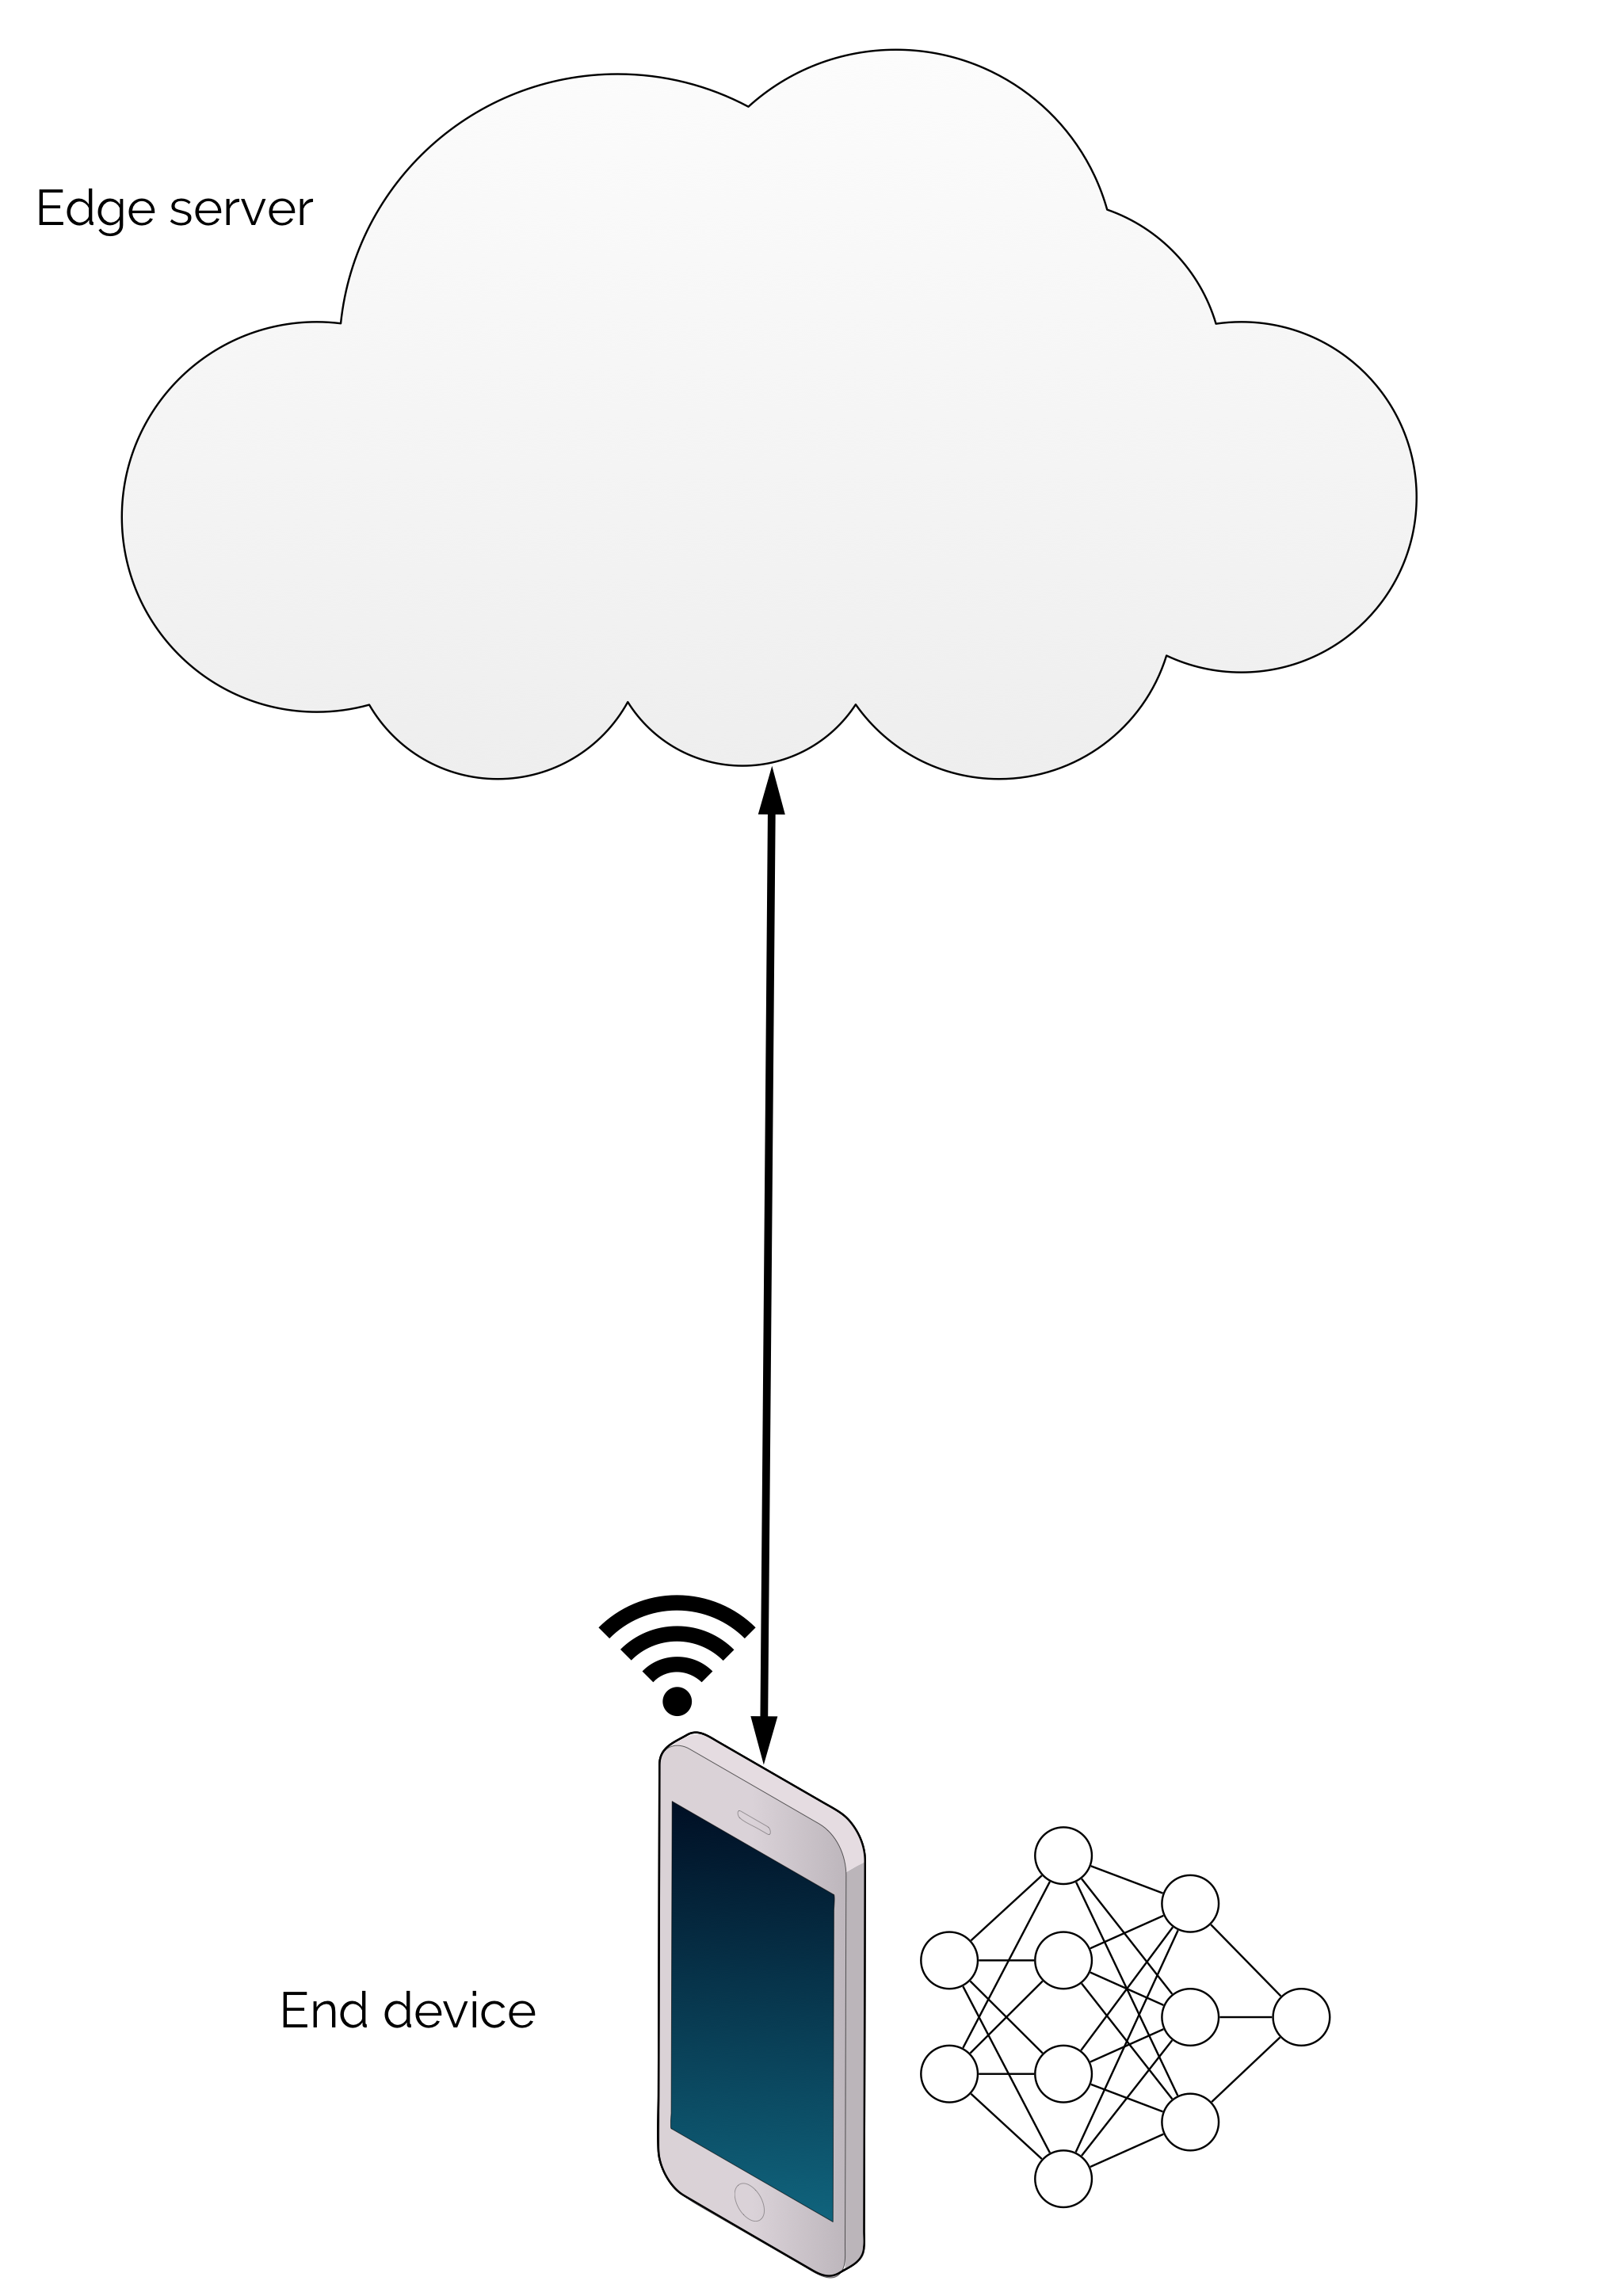
\includegraphics[width=.2\linewidth]{figures/models/device}}
	\subfloat[Edge-based\label{fig:edge-based}]{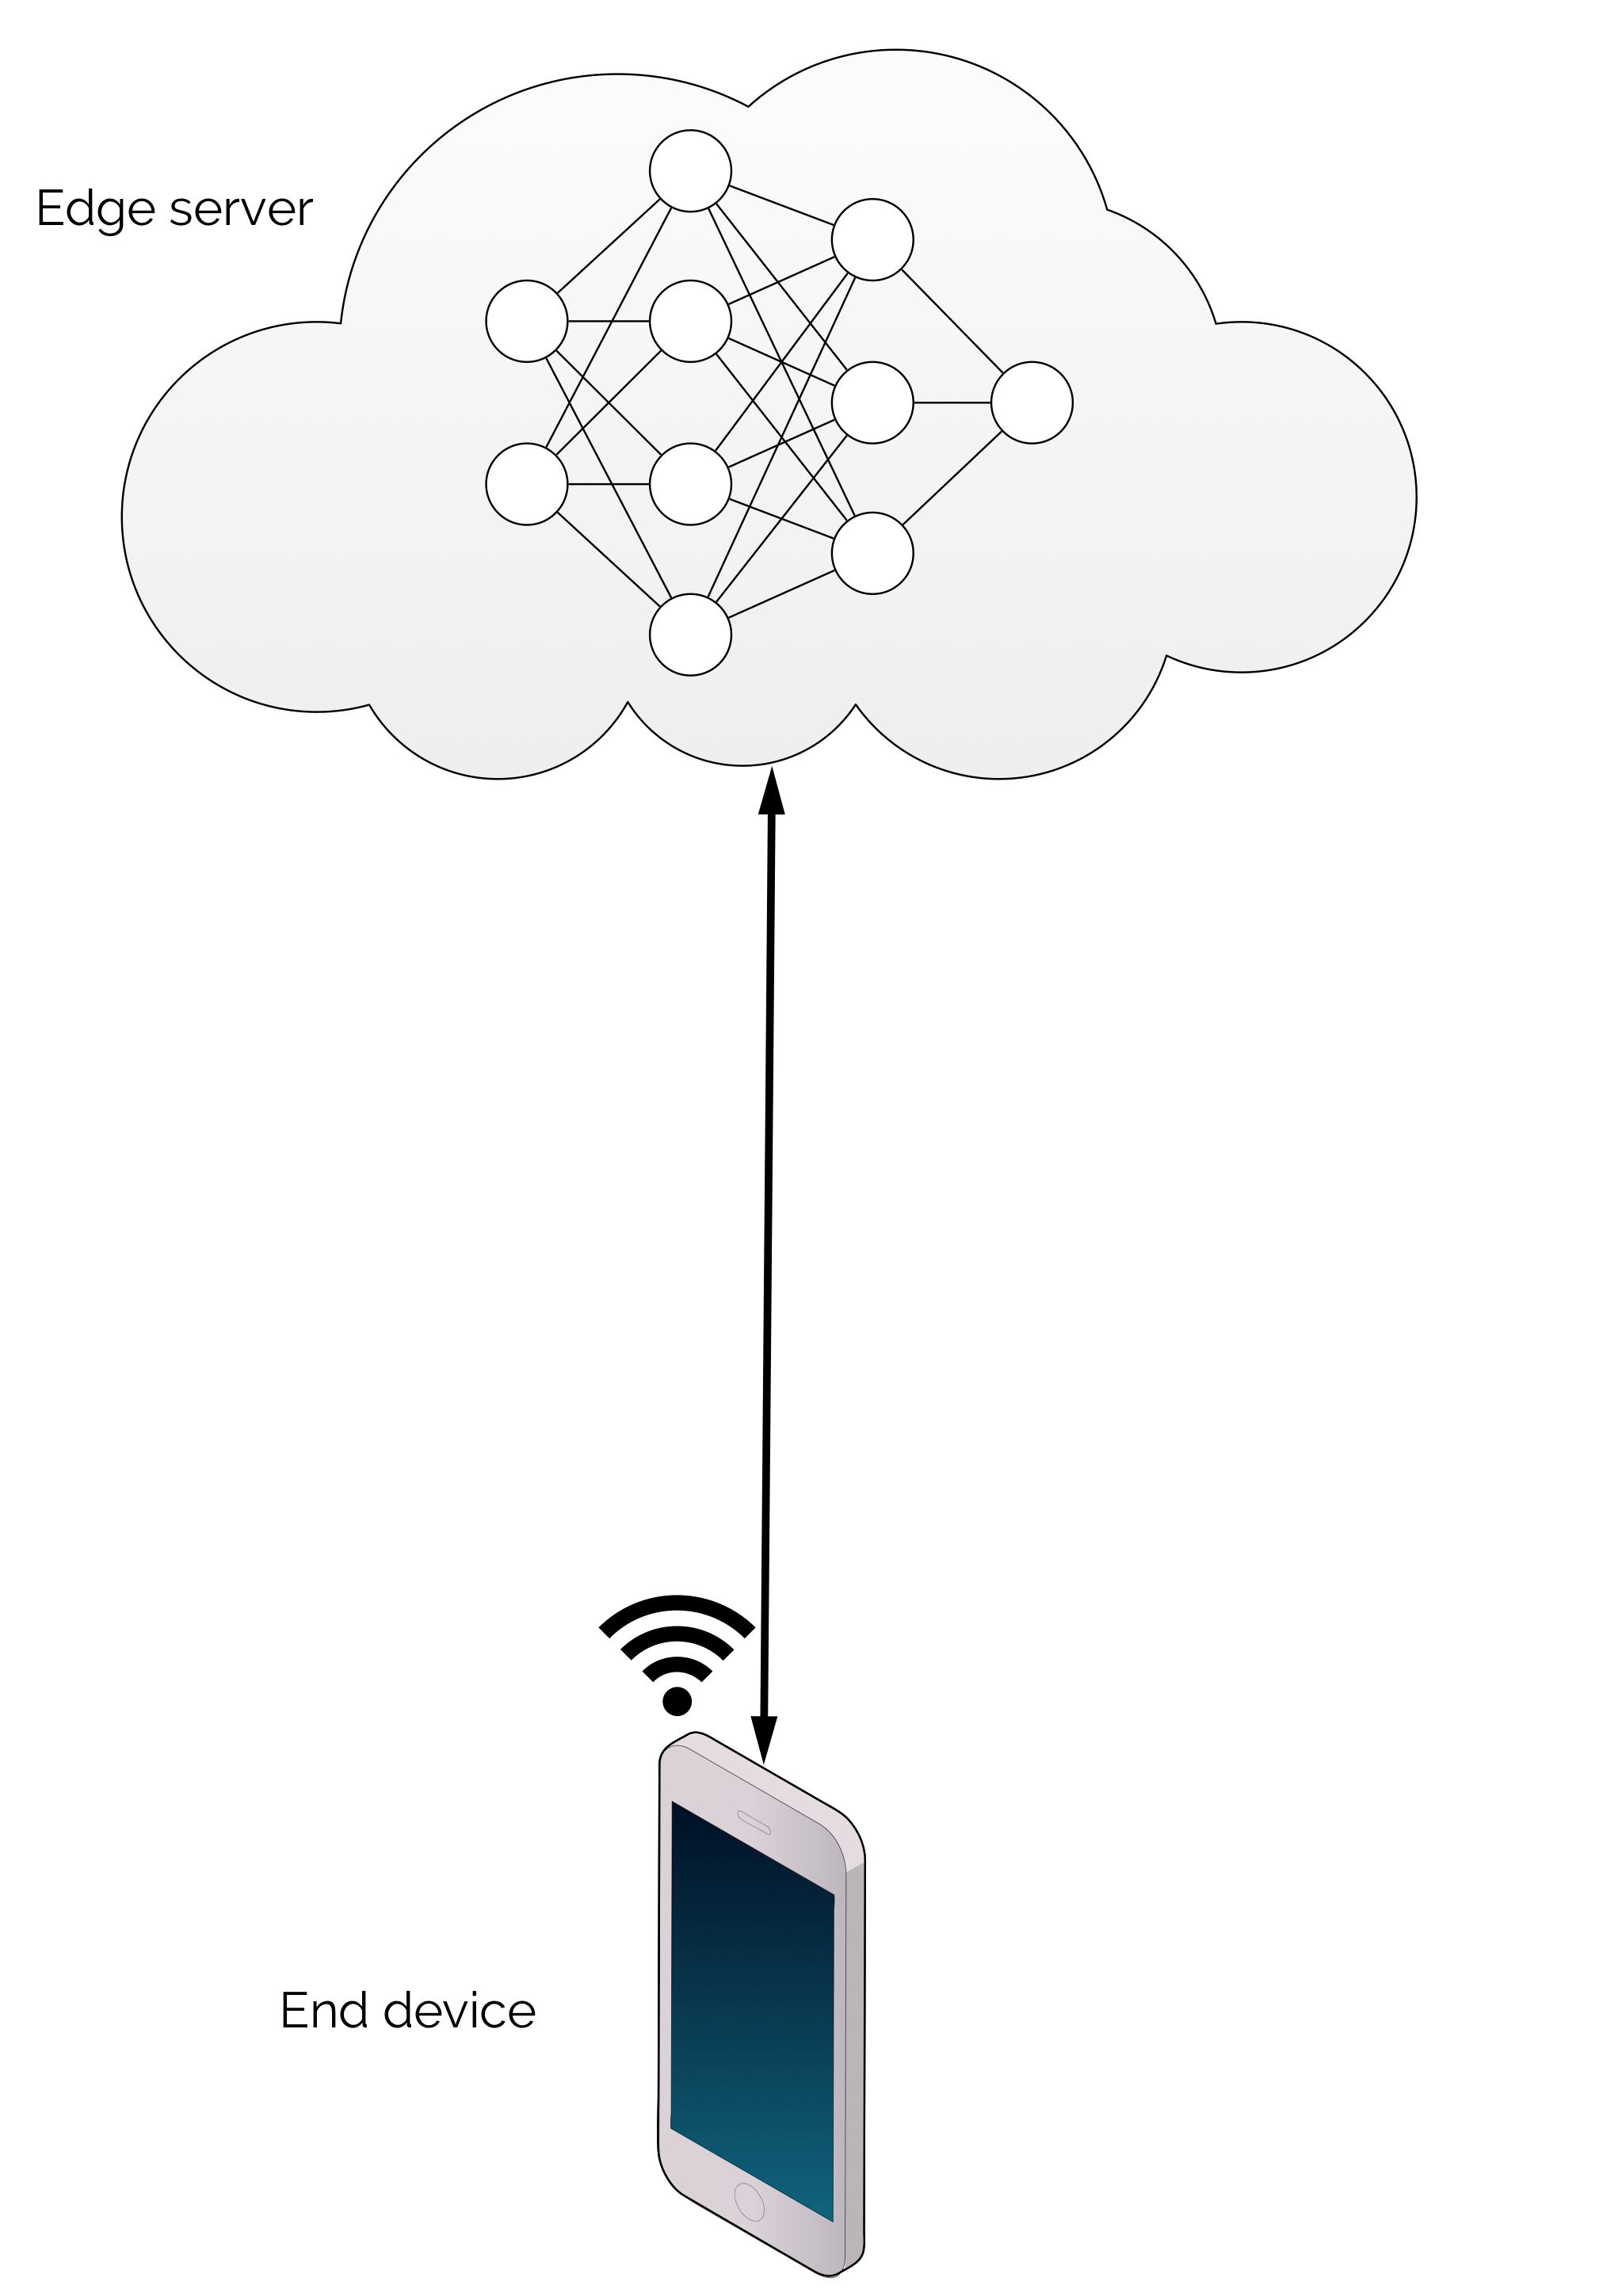
\includegraphics[width=.2\linewidth]{figures/models/edge}}
	\subfloat[Edge-Device mode\label{fig:edge-device-mode}]{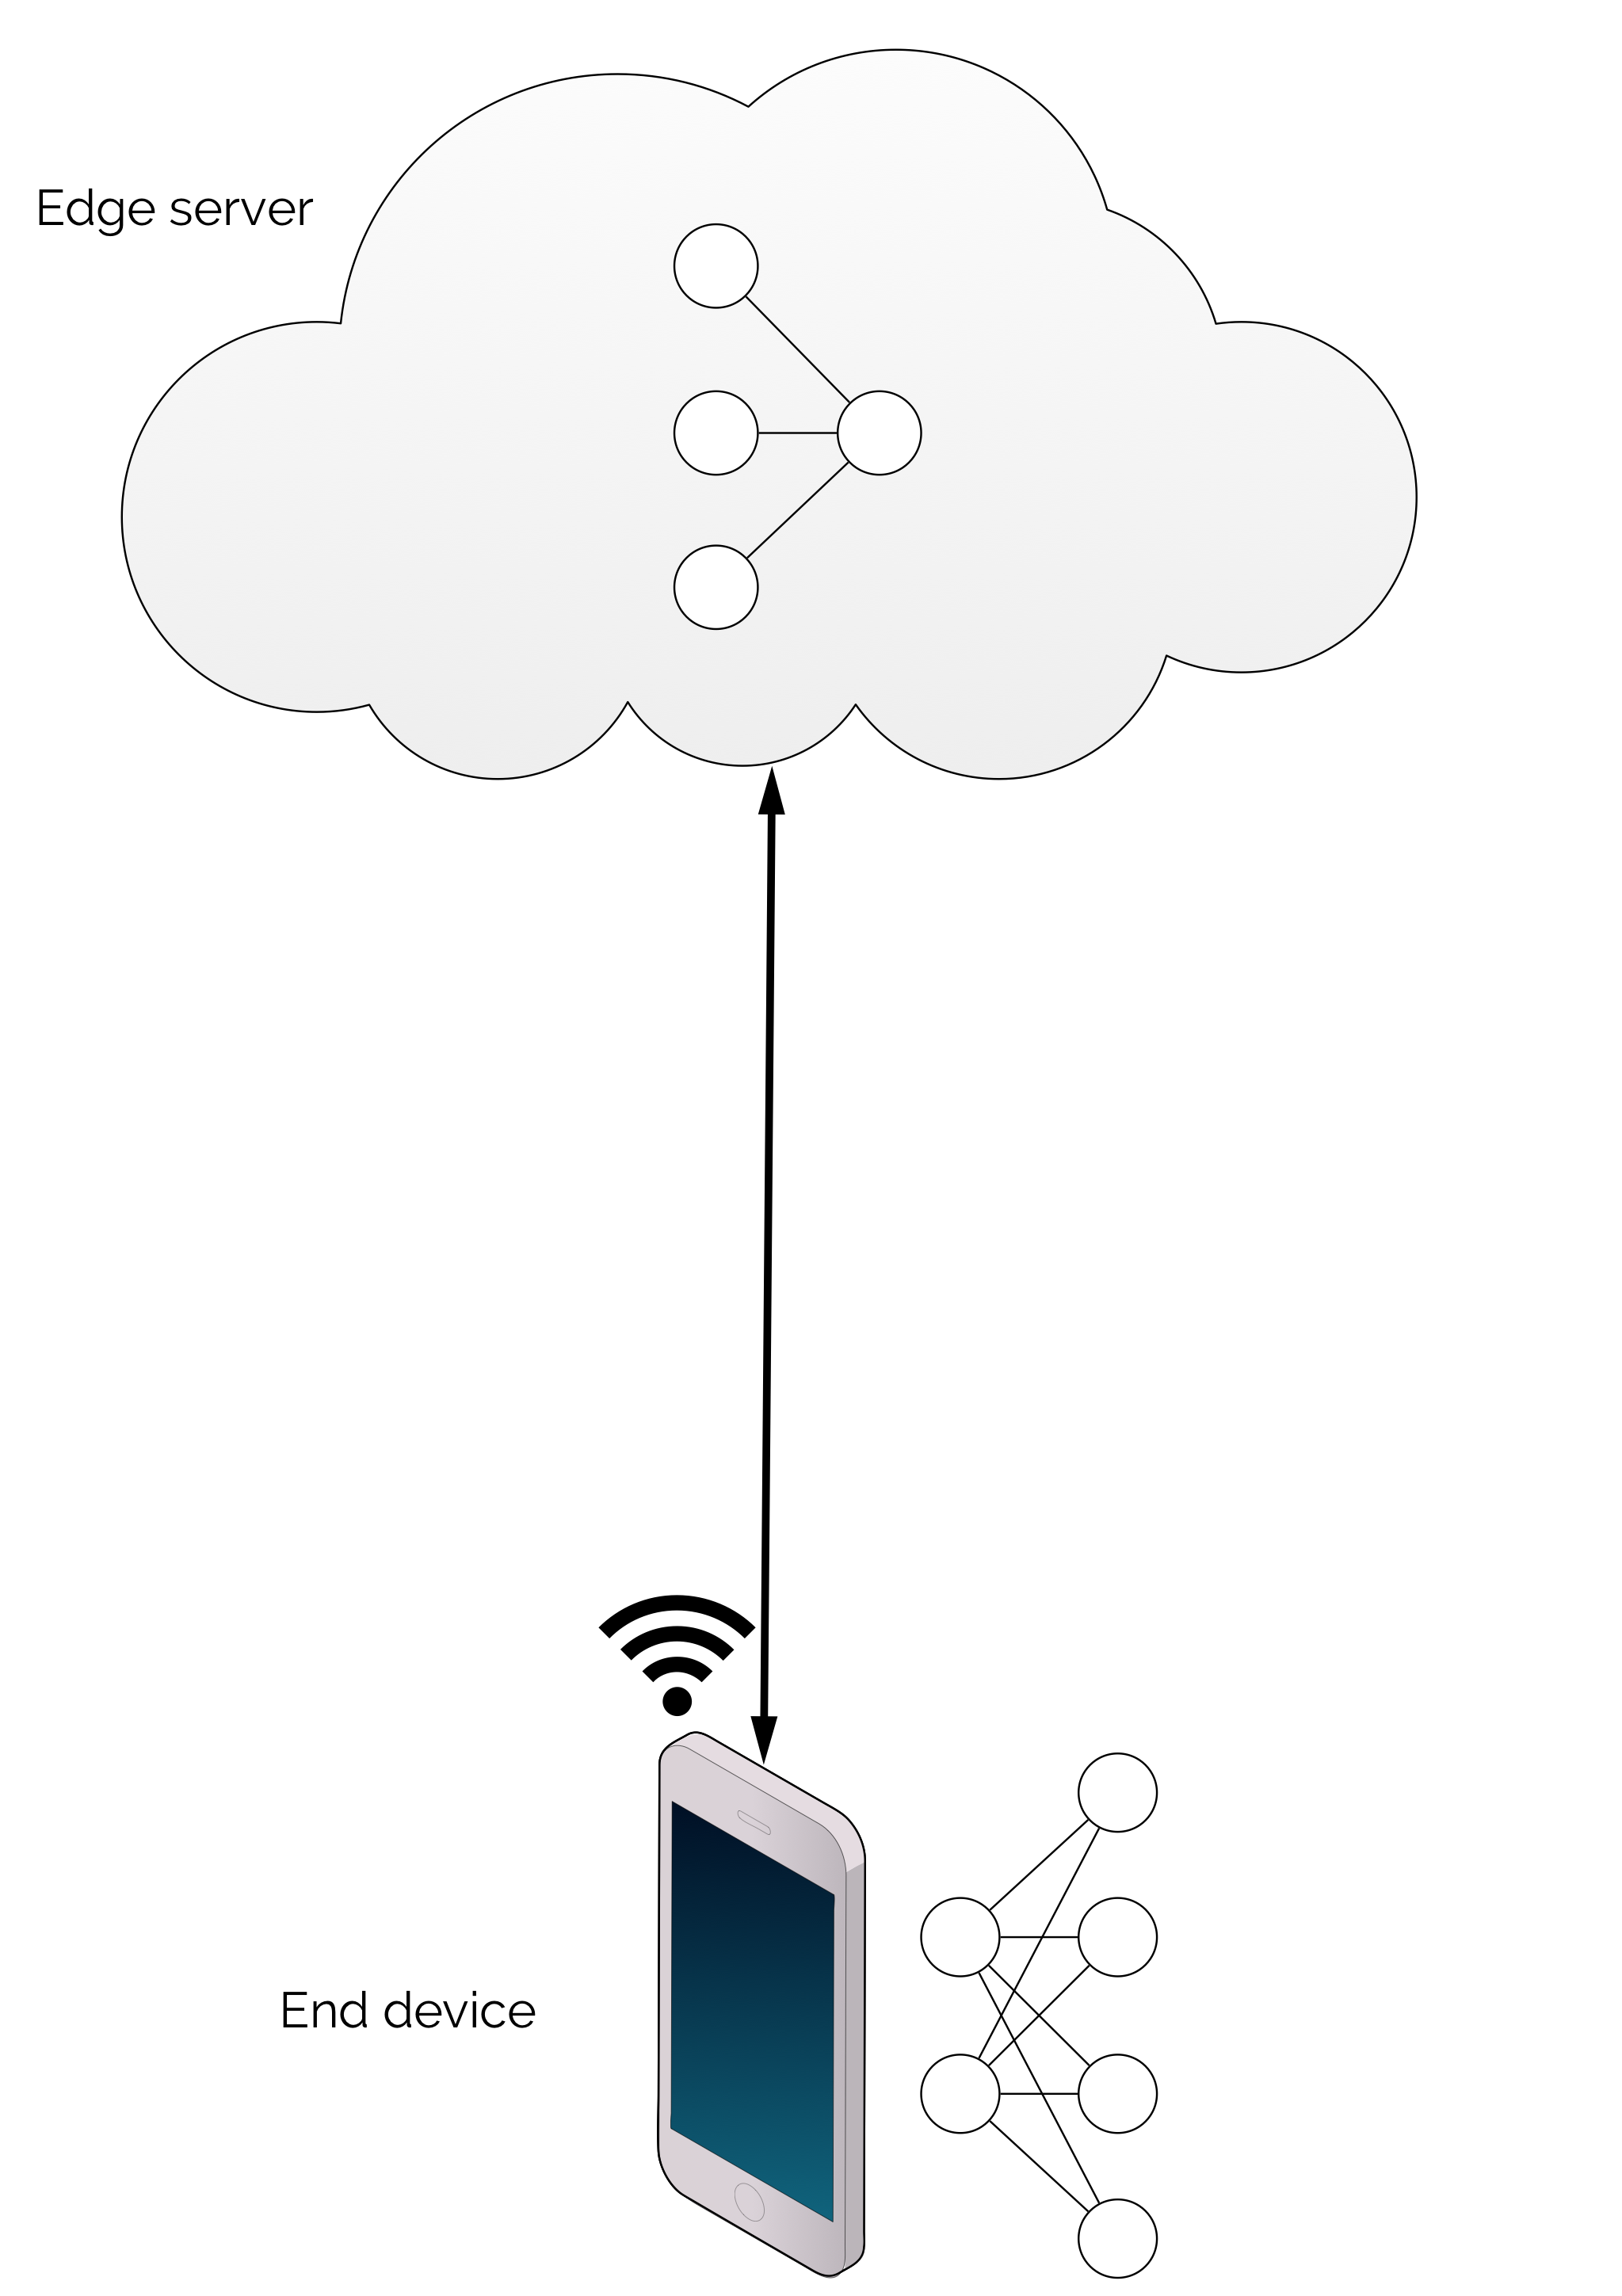
\includegraphics[width=.2\linewidth]{figures/models/edge_device}}
	\subfloat[Edge-Cloud mode\label{fig:edge-cloud-mode}]{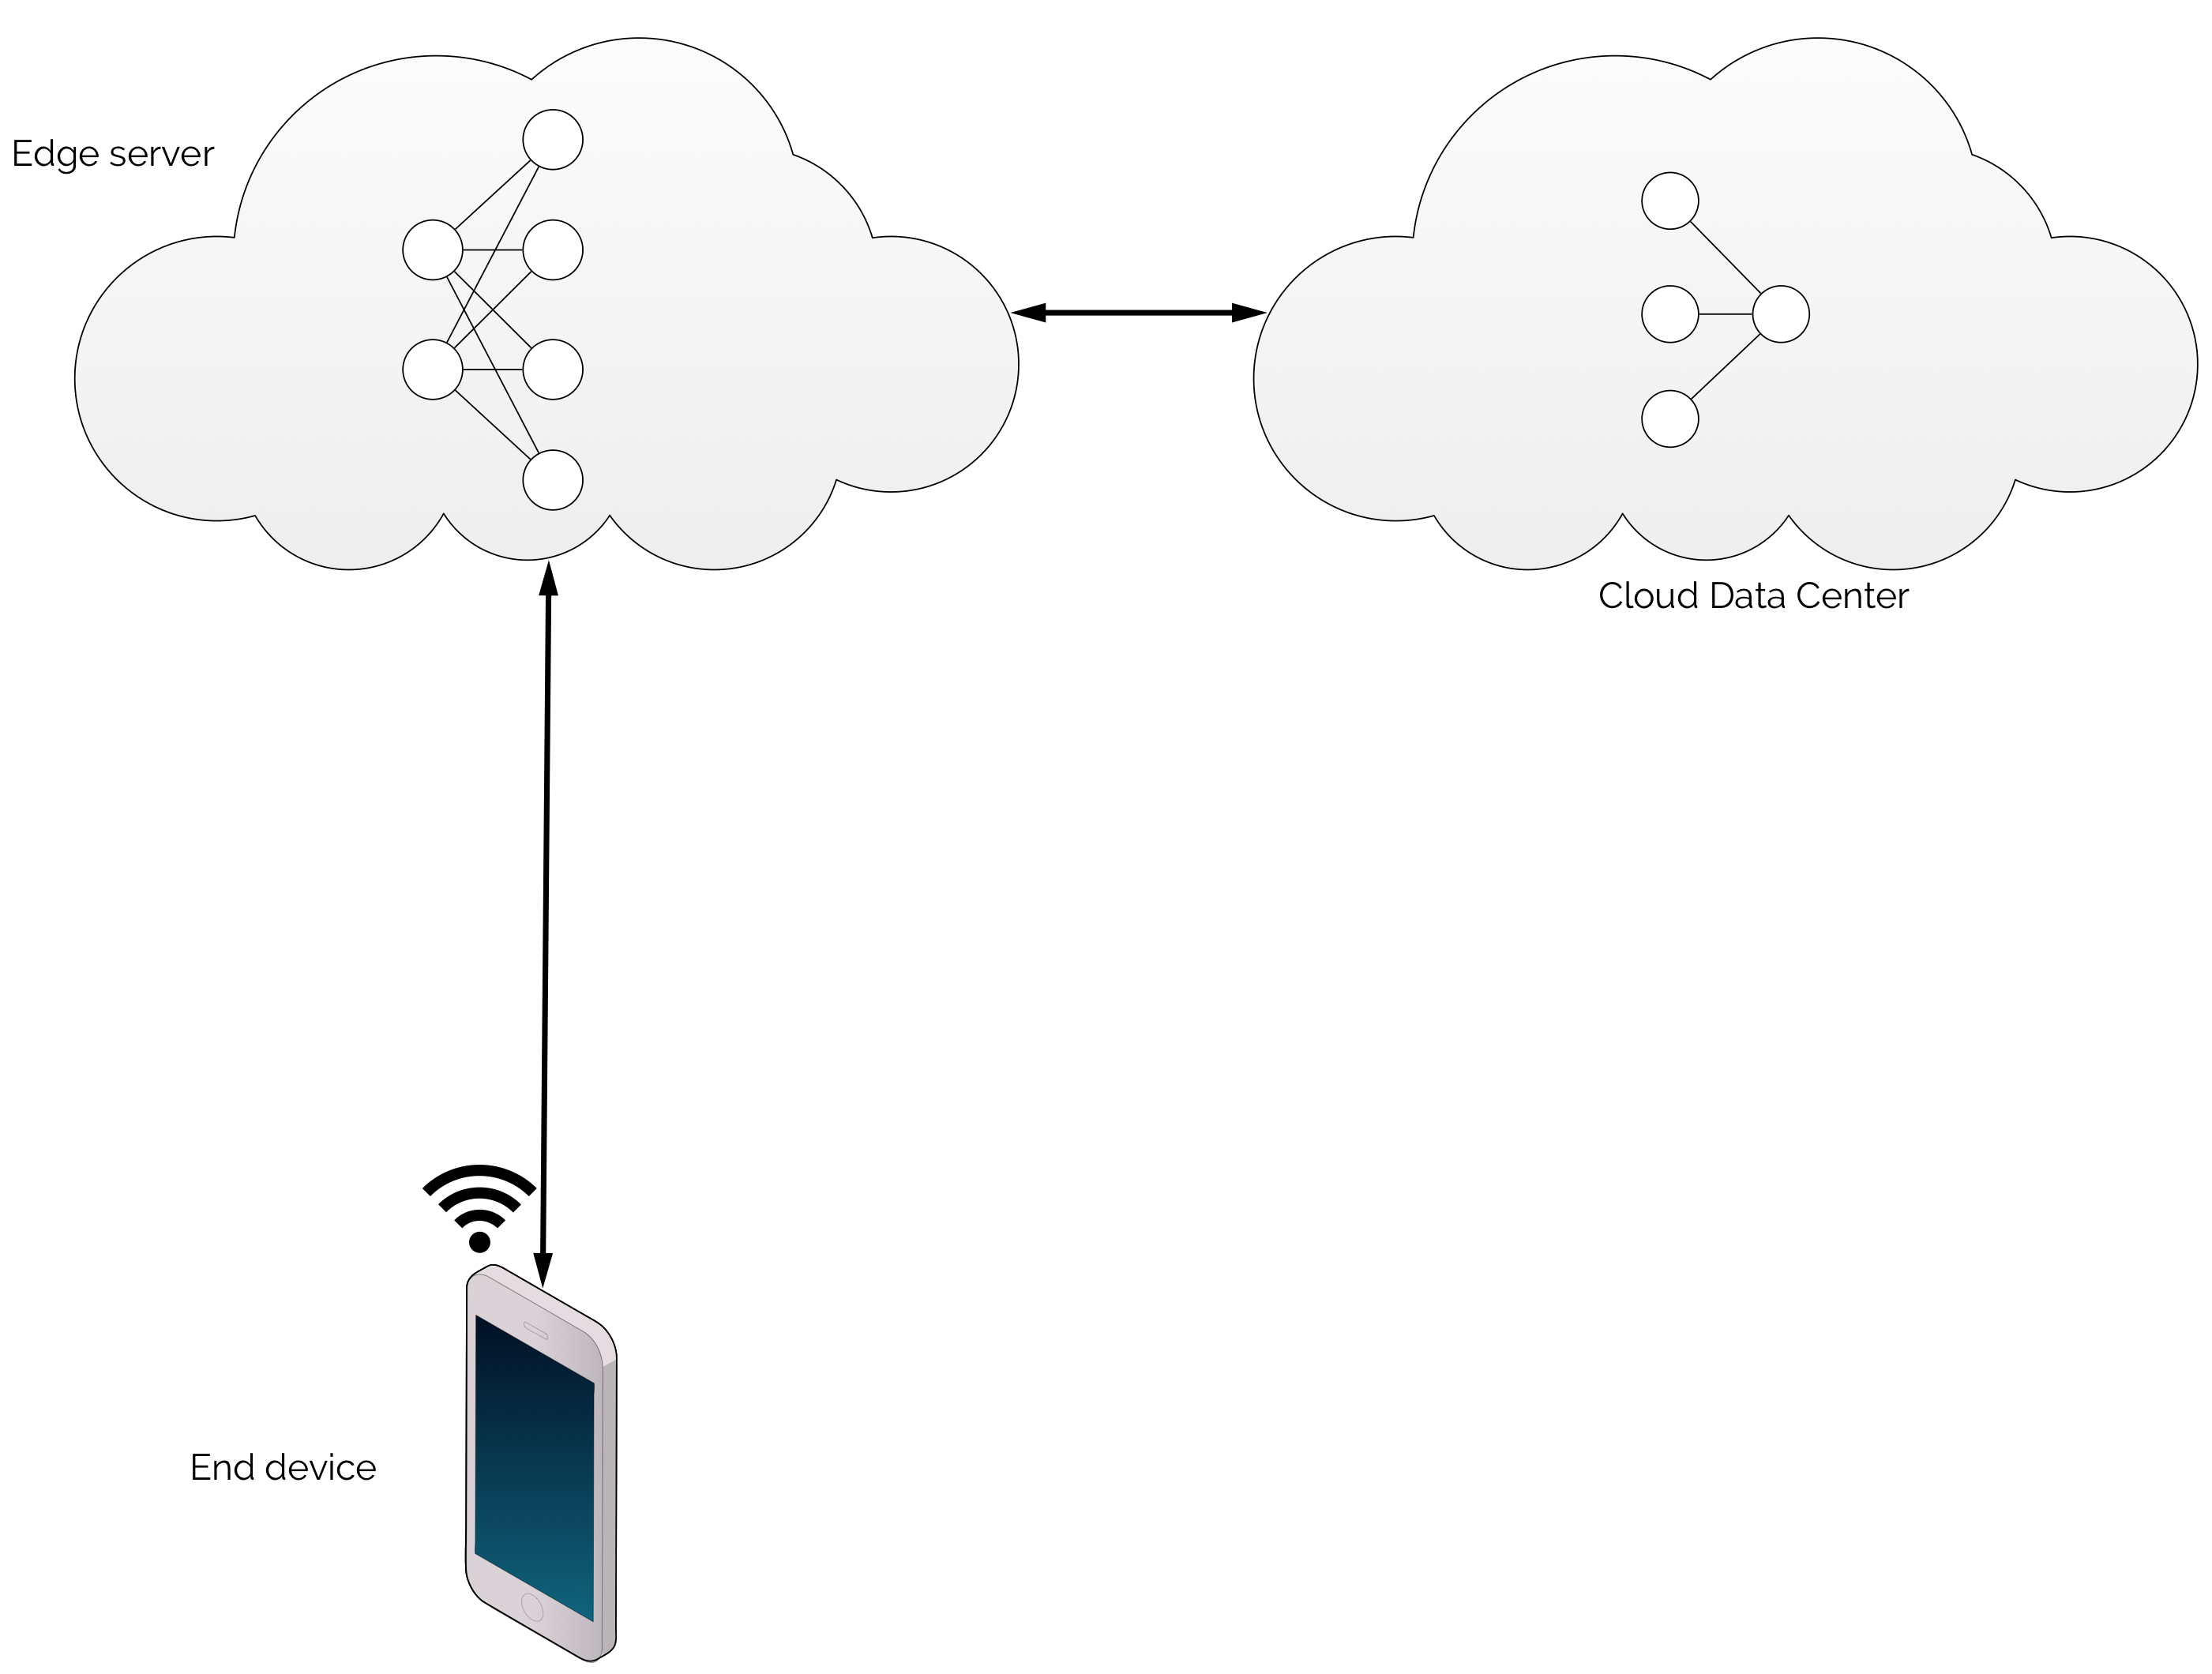
\includegraphics[width=.37\linewidth]{figures/models/edge_cloud}}
	\caption[Edge-centric arcchitectures]{Edge Archtitectures: \protect\subref{fig:device-based} device only execution, \protect\subref{fig:edge-based} edge only execution,\protect\subref{fig:edge-device-mode} edge and device partially execution, \protect\subref{fig:edge-cloud-mode} edge and cloud partially execution. }
\end{figure}

\begin{description}
	\item[Device-based Mode] end device obtain model from edge server. The end-device then acquires input data and performs model inference. Since all computation is done on the end device, performance is solely reliant on the end device's computing resources.  
	\item[Edge-based Mode] end device acquires input data. The input data is transferred to an edge server, which performs model inference and send the prediction results to the end device. The performance relies on edge server computing resources and network bandwidth.
	\item[Edge-Device Mode] end device acquires input data and performs partially model inference. The intermediate data is transferred to an edge server which finalizes model inference. The performance relies on end device's and edge server computing resource, network bandwidth and edge server workload. 
	\item[Edge-Cloud Mode] resemble edge-device mode, however the model inference task is now partitioned between edge server and cloud data centers. The model is now reliant on edge server and data center computing resources, but even more reliant on \gls{wan} transmission rate between edge and cloud. 
\end{description}

\subsection{Performance Metrics}

The aim of edge intelligence is to accommodate certain performance metrics:

\begin{description}
	\item[Latency] is defined as the overall time of the inference process, including from data is generated at the device, data transmission, preprocessing, model inference and postprocessing. For \gls{ei} real-time application, such as \gls{ar}/\gls{vr}, where stringent deadlines requirements must be met e.g. 100ms \cite{bibid}. Latency is affected by several factors; computing resources, data rate, model architecture and execution.
	
	\item[Accuracy] is defined as the ratio of correctly predicted input samples from the total number of inputs. 
	\begin{align*}
		\alpha = \frac{n_c}{N}
	\end{align*}
	Accuracy requirements are dependent on the \gls{ei} application, for instance autonomous vehicles require extreme accuracy with extremely low latency. The essential trade-off is how accurate a model can we use while still satisfying latency demands.  
	
	\item[Energy efficiency] end devices are typically battery powered, thus applications must be optimized for energy efficiency. Energy efficiency for offloading application is finding the right trade-off between computation and communication. The hardware of end-devices play a crucial role, it may be more sensible to have a device-only execution, if it's a powerful \gls{gpu} enabled mobile device. If it's a \gls{cpu}-only device, then naively offloading entire model inference may introduce a communication overhead in poor communication environments, hence a partial execution model between end-device and edge may be optimal. 
	
	\item[Communication overhead] is introduced whenever inference is offloaded for remote computation. The energy impact of communication is highly dependent on the wireless technology, as is the overall latency. Cloud-offloading is highly dependent on unreliable and expensive \gls{wan} connection to a cloud data center, as high variation in network traffic and server workload occurs. Edge-offloading mitigates the impact of communication overhead, by solely depending on a more reliable \gls{lan} network connection to edge servers.  
	 
	\item[Privacy] data generated by end devices might be confidential, hence not allowed to be processed by a data center unless confidentiality can be guaranteed. Privacy relies on how data is process within the \gls{ei} application. Offloading model input data, may be susceptible to interception, as it may be well understood by an adversary, however offloading intermediate data with no apparent meaning for humans may help improve the confidentiality of data.    
	
	\item[Memory footprint] reducing memory footprint of \gls{dnn} inference is important especially for mobile device. The mobile device do not have dedicate \gls{gpu} memory, hence \gls{dnn} application will have to compete with other applications running on both \gls{cpu} and \gls{gpu}. The resource hungry \gls{dnn} application will drain battery resources and potentially harm performance of coexisting applications.   
\end{description}

\subsection{Enabling technologies (related work?)}

This work is mainly concerned the accuracy-latency trade-off for inference in \gls{ei} applications and services. Thus, it will primarily address technologies regarding these performance metrics, and refer to the survey for a broader perspective on all of the performance metrics for \gls{ei} applications and services. The centralized device-based and edge-based architectures are addressed by common \gls{dl} literature. The distributed inference models for \gls{ei} is a fairly recent and promising field of research for truly enabling \gls{ai} applications and services.

Technologies for distributed \gls{dnn} inference includes:

\begin{description}
	\item[Model Compression] description \cite{courbariaux_binaryconnect:_2015}
	\item[Model Partition] Splitting a model to run on both cloud for Edge-Device mode is an inherent nature of sequential \gls{dnn}s, that at any layer can be stopped. The intermediate output are transferred over the network and continued at the next layer on an edge server. Neurosurgeon \cite{kang_neurosurgeon:_2017} is a lightweight partitioning scheduler, that uses knowledge of the individual layers of the \gls{dnn} to effectively reduce inference latency. Communication latency is the bottleneck in an offloading application, hence a smaller representation of the input data is needed, however the layers producing a smaller output than the original input typically lies deep within the network. Neurosurgeon construct regression models for layer execution time and  output data size of the layers of a \gls{dnn}, to decide the best partition of the \gls{dnn} based on networking condition. The work is based on \gls{mcc} and shows, that the conventional cloud-only approach is insufficient due to different networking technologies and mobile device is becoming \gls{gpu} enabled. 
	% Evidently moving computation to the edge reduces the communication latency. 
	
	Another effort to reduce communication overhead of network splitting is adding feature compression of intermediate features before offloading to cloud \cite{choi_deep_2018}. The paper shows, that lossless compression have no impact on accuracy, but also with limited bit saving. Lossy compression on the other hand results in 70\% bit savings, however also affect accuracy and require compression-aware training to compensate. The follow up paper \cite{choi_near-lossless_2018} propose compression techniques for deep features and achieve significant better bit saving, than conventional image compression algorithms. 
	
	BottleNet \cite{eshratifar_bottlenet:_2019} is a novel neural network module. Client-side it consists of a reduction unit and a compressor and server-side of a decompressor and restoration unit. The reduction unit creates a smaller representation of intermediate result by applying spatial- and channel-wise convolution. The compressor uses lossy \gls{jpeg} compression, that are decompressed server-side. The restoration unit apply deconvolution to restore the intermediate feature back to the required dimensionality for the next layer in the network. BottleNet is able to achieve 84$\times$ bit savings compared to cloud-only approach with less than 2\% degradation of accuracy caused by lossy compression. Under good networking condition, the evaluation of BottleNet shows, that the best split is after the first convolutional layer, which give a 8$\times$ speed up compared to cloud-only approach using WiFi.
	
	\item[Model Early-Exit] BranchyNet
	
	Note: \cite{park_big/little_2015} examines other ways to define exiting threshold. Although it is a model selection approach.
	 \cite{teerapittayanon_branchynet:_2016} proposed by \citeauthor{teerapittayanon_branchynet:_2016} is an early exiting framework for fast inference of a \gls{dnn}. The work states, that typically samples can be accurately classified using less \gls{dnn} layers which can improve the inference time, if a sample cannot be classified with proper confidence more layers can be used to obtain a more confident prediction. The framework shows promising results of reduced inference time, added regularization via joint optimization of exiting points and mitigation of vanishing gradients. The result are based on three well-known \gls{dnn} architectures; LeNet \cite{lecun_lecun-98.pdf_1998}, AlexNet \cite{krizhevsky_imagenet_2017} and ResNet \cite{he_deep_2015}, modified to implement the BranchyNet framework, and to accommodate the MNIST \cite{lecun_mnist_2010} and Cifar-10 \cite{krizhevsky_cifar-10_nodate} datasets.  
	
	The architecture is suited for \gls{p2p} applications and adaptive to fit any aforementioned \gls{ei} architectures, as it supports network splitting. It can run Device-based, Edge-based and be split to run distributed on device, edge or cloud.
	
	\gls{ddnn} \cite{teerapittayanon_distributed_2017} also proposed by \citeauthor{teerapittayanon_distributed_2017}, extend upon BranchyNet,  to  create a distributed computing hierarchy over cloud, edge and end devices. The work shows benefits from distributed computing to provide fault tolerance when end devices are failing.
	
	\item[Edge Caching] description
	\item[Input Filtering] description
	\item[Model Selection] description
	\item[Support for Multi-Tenancy] description
	\item[Application-specific Optimization] description
\end{description}



\section{Training Settings}



\paragraph{Optimizer}

The weights of \gls{dnn}s are typically trained using a variant of \gls{sgd}. Some more about \gls{sgd} \cite{goodfellow_deep_2016}.

\gls{sgdr} \cite{loshchilov_sgdr:_2016} is a variant of \gls{sgd}, the method have shown faster convergence on a number of datasets, due to its ability to escape local minimas. It follows a cyclic learning rate schedule in contrast to former decaying learning rate schedules. It has shown, in general, to perform better than adaptive optimizers such as Adam \cite{kingma_adam:_2014}, which implement adaptive learnining rate to avoid being stuck in local minimas. 

\gls{sgdr} uses an aggressive cosine annealing schedule with warm restarts. Figure \ref{fig:cosineannealing} illustrates the learning rate schedule.

\begin{figure}
	\centering
	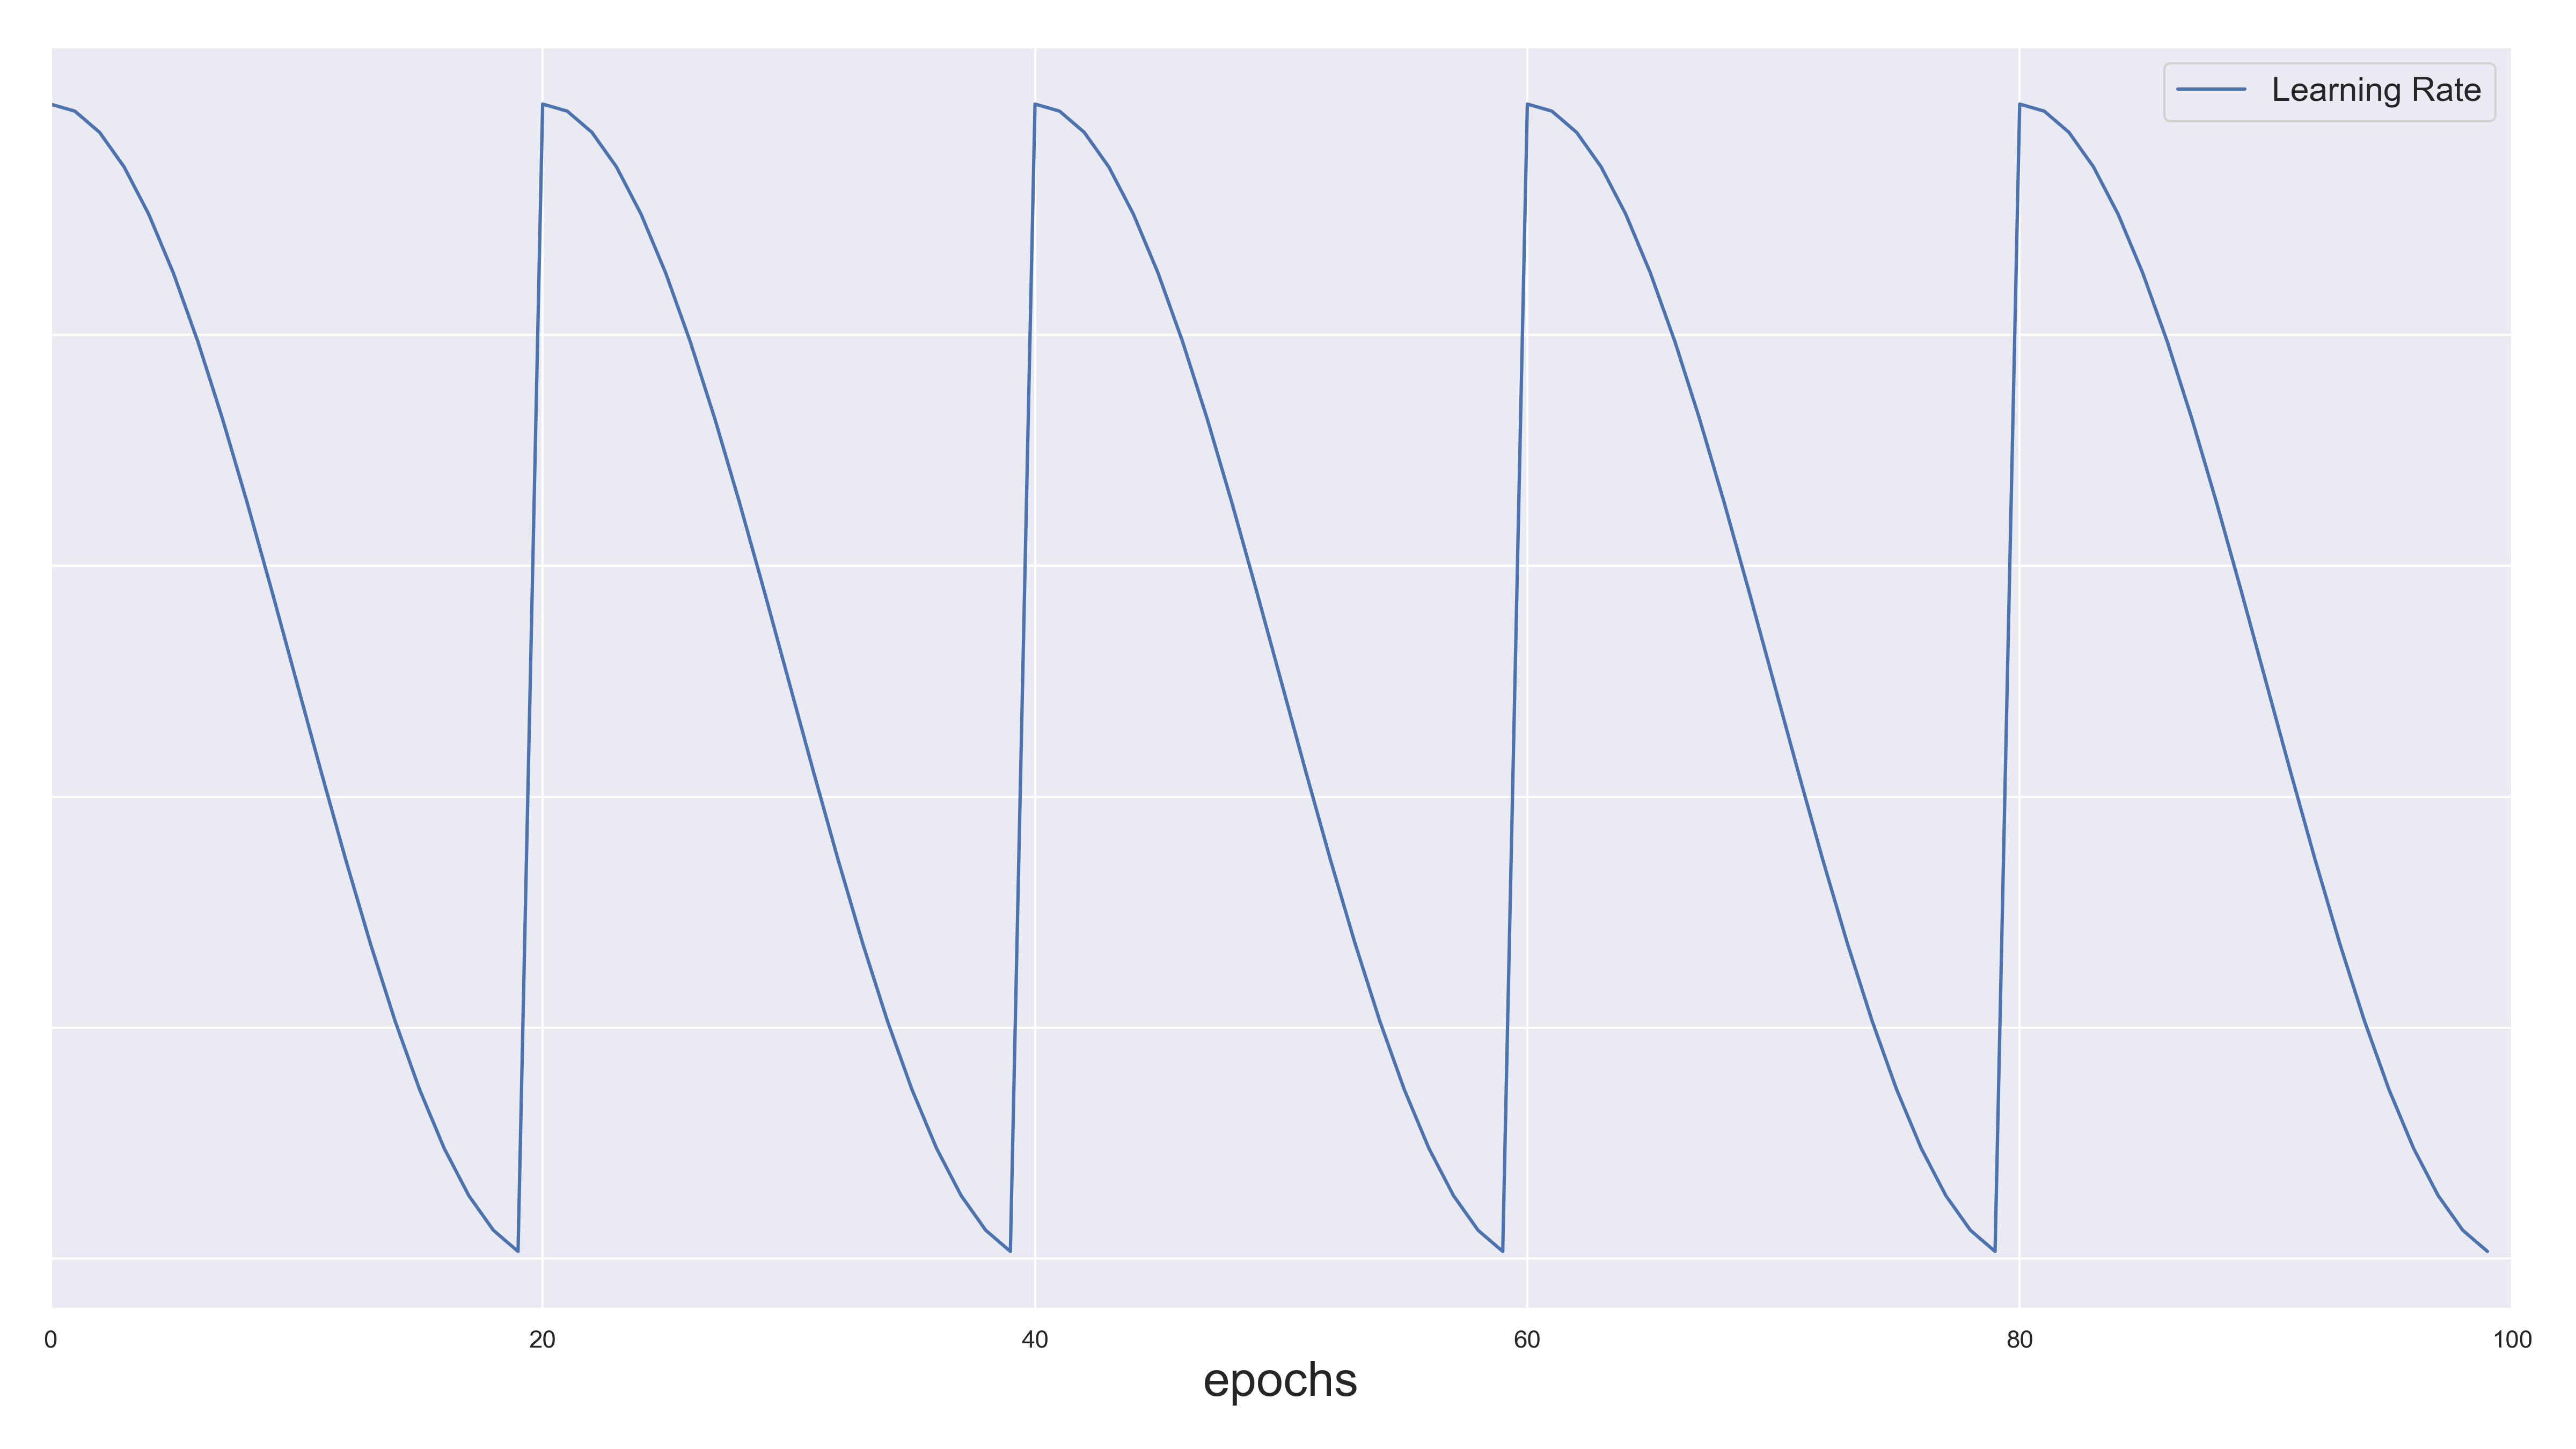
\includegraphics[width=.7\linewidth]{figures/lr.png}
	\caption[Cosine Annealing Learning Rate]{Cosine Annealing Learning Rate} \label{fig:cosineannealing}
\end{figure}

\paragraph{Batch Size}

Batch Size are recommend to be between 1 and a few hundreds \cite{bengio_practical_2012}, to better utilize \gls{gpu}s a batch size in the power of 2 gives better runtime, e.g. 32 to 256 \cite{goodfellow_deep_2016}. Larger batch sizes have been driving by advancements in parallelism \cite{dean_large_2012}, which can improve the training time, however smaller batch size, have shown better generalization performance due to a regularizing effect \cite{masters_revisiting_nodate}, which especially large model, that tends to overfit can benefit from \cite{goodfellow_deep_2016}. 

In this project a single \gls{gpu} GTX1080 with 8Gb memory is used to train the models. A batch size of 16 is chosen for all \gls{dnn} training sessions, which is the maximum power of 2 possible with the computational budget, as the typical choice of 32 samples in a batch caused memory exhaustion. A batch size of 16 should be adequate and still provide decent training times. 

\paragraph{Datasets}

\gls{min100} is a subset of the \gls{ilsvrc2012} dataset \cite{russakovsky_imagenet_2015} created for this project, to reduce training time from several weeks to only days on available hardware. The sub-setting is inspired by MiniImageNet \cite{vinyals_matching_2016}, that uses a subset of 100 classes with 600 samples for each class. \gls{min100} contains 100 out of 1.000 randomly sampled classes, which gives 127.300 out of 1.2m training samples and 5.000 out of 50.000 validation samples. A full list of classes are found in the appendix. 

Compared to other sufficiently dense classification datasets e.g \gls{tinyimagenet} \cite{li_cs231n:_2018}, \gls{cifar10} and \gls{cifar100} \cite{krizhevsky_cifar-10_nodate}, the image sizes of these datasets are respectively $(64\times 64$), $(32\times 32)$, $(32\times 32)$ pixels, all of which are considered too small  for this project. Other datasets such as MS COCO and Pascal VOC are better suited for object detection/segmentation, as images are not cropped to only focus on a single object, thus too challenging for classification. In fact Pascal VOC was initially tested, the model however, clearly overfitted the training data due to data sparsity. 

\paragraph{Image Augmentation}

A models ability generalize a specific classification problem has a close connection with the number of available training samples. Data augmentation haven proven to be powerful tool in order to virtually create more training data \cite{perez_effectiveness_2017}. Enlarging a training dataset by data augmentation can help create new versions of an image, that are different from but still similar to the original image, without actually having to acquire and annotate new samples \cite{goodfellow_deep_2016}.  

\begin{figure}[H]
	\centering
	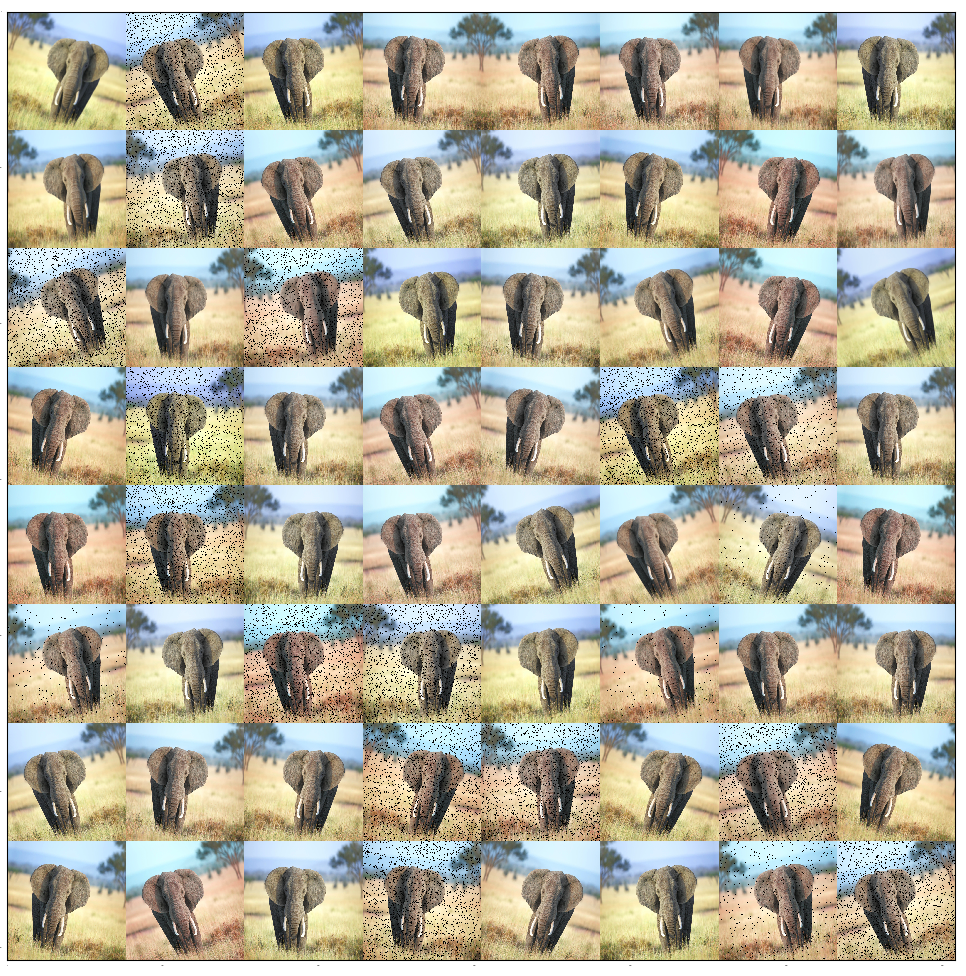
\includegraphics[width=.7\linewidth]{figures/augmentation/augmentation_high_resolution.png}
	\caption[Image Augmentaion Example]{Image Augmentation of an elephant}
	\label{fig:augmentation}
\end{figure}

Image augmentation involves transformations using tools from image processing to randomly apply noise injection, and color space transformations including contrast and saturation distortions, as well as geometric transformations, such as simple transformations of flipping the image to more complex affine transformations to create different image perspectives \cite{shorten_survey_2019}. Figure \ref{fig:augmentation} shows 64 random augmentations of an image of an elephant. 

New methods have been proposed where image transformations are learned to improve generalization e.g. AutoAugment \cite{cubuk_autoaugment:_2018}. 

Other methods involves actually enlarging the training dataset by synthetically creating more data using a \gls{gan}. \gls{gan}s can help overcome limited data given the available training data or a 3D model, by artificially constructing new samples in different background, light setting and from alternate perspectives.

Methods that do not cover enriching the available training, but alters the learning procedure are called regularization and covers; weight decay, dropout, batch normalization etc.

\paragraph{Transfer Learning}

Transfer learning is the procedure of using a pre-trained model to train on a new dataset. Under the assumption, that features learned on one image dataset can be reused for another dataset \cite{yosinski_how_2014}. Transfer learning can reduce the needed time to learn general features and possibly learn better ones. Typically models have been pre-trained on the ImageNet dataset. The density of the dataset, enables model to learn general features suitable for many other domains \cite{kornblith_better_2019}. Transfer learning are especially suited for when the new data domain is of limited quantity and when the similarities between the two data domains are strong. If the similarity is less strong a model can be partially trained, the shallow layers containing general features are frozen and only the deeper layers with more specialized features are fine-tuned for the new data domain \cite{li_cs231n:_2018}. 
